
Нуклеосомы представляют собой наиболее распространенные комплексы белок-ДНК у эукариот, которые обеспечивают уплотнение геномной ДНК и участвуют в регуляции транскрипции, репликации и репарации ДНК. Детали позиционирования ДНК на нуклеосоме и конформации ДНК могут являться важными регуляторными сигналами. Метод футпринтинга комплексов белок-ДНК гидроксильными радикалами -- это химический метод, который позволяет исследовать организацию нуклеосом в растворе с высокой точностью, недостижимой другими методами. В этой работе мы предлагаем метод интегративного моделирования для построения атомистических моделей нуклеосом с высоким разрешением на основе экспериментов по гидроксильному футпринтингу. Наш метод точно определяет положение ДНК на нуклеосоме путем на основе данных футпринтинга для обеих цепей ДНК, используя свойства псевдосимметрии нуклеосомы. Мы провели эксперименты по гидроксильному футпринтингу с высоким разрешением для центромерных нуклеосом \textit{Saccharomyces cerevisiae}, структура которых является предметом дискуссий. Мы охрактеризовали эти структуры, используя наш подход интегративного моделирования. Наша модель обеспечивает основу для дальнейшего понимания взаимодействия между белком Cse4p и последовательносями аденинов (A-трактами), важными для функции центромеры в пекарских дрожжах.

\subsection{Введение}
Нуклеосомы - это элементарные строительные блоки хроматина, включающие сегмент ДНК, связанный с октамером гистоновых белков (H3, H4, H2A, H2B - по две копии каждого) \cite{kornberg_chromatin_1974-1}. Кор нуклеосомы (называемый, кором нуклеосомы или NCP) состоит из 145–147 п.н. ДНК, обернутых в виде $\sim$ 1,7 левых сверхспиральных витка вокруг октамера \cite{luger_crystal_1997} (рис. \ref{fig:p5:p5_2_f1}). Хотя общая структура нуклеосомы хорошо охарактеризована \cite{tan_nucleosome_2011}, каждая конкретная нуклеосома может значительно отличаться от своих аналогов за счет вариаций в последовательности ДНК, включения альтернативных вариантов гистонов \cite{draizen_histonedb_2016,shaytan_nucleosome_2015}, их посттрансляционных модификаций \cite{gardner_operating_2011} и взаимодействий с другими белками \cite{xiao_nonhistone_2011,becker_nucleosome_2013}. Эти изменения и вариации часто влияют на доступность и конформацию ДНК, которые, в свою очередь, модулируют основные процессы в хроматине, такие как транскрипция, репликация, репарация ДНК и т. д. \cite{gaykalova_structural_2015,luger_new_2012}. Смещение положения ДНК в нуклеосоме только на одну пару оснований приводит к изменениям в ее ротационном позиционировании примерно на 36 градусов, что может быть достаточно, чтобы повлиять на связывание многих белков с нуклеосомами, считывающими последовательность ДНК (например, пионерские факторы транскрипции \cite{iwafuchi-doi_pioneer_2014,cui_rotational_2014}). Следовательно, детальная структурная характеристика нуклеосом имеет большое значение. Атомные структуры отдельных нуклеосом получались с помощью рентгеновской кристаллографии \cite{tan_nucleosome_2011}. Однако этот метод требует очень много времени и во многих случаях сильно ограничен ограничениями по кристаллизации, составу и конформации нуклеосомы, потенциально приводя к конформациям, отличным от тех, которые могут быть в растворе. Поэтому очень востребованы точные и универсальные методы характеристики структур нуклеосом.
В лаборатории широко используются определенные биохимические методы для быстрой характеристики доступности и расположения ДНК на нуклеосомах в растворе. В этих методах используется визуализация ``следа'' белков на ДНК - разрезание ДНК ферментами или химическими веществами. Эти методы позволяют картировать взаимодействия белок-ДНК и охарактеризовать конформацию ДНК вдоль последовательности ДНК. Метод гидроксил-радикального футпринтинга (HRF) признан методом, обеспечивающим наивысшее разрешение благодаря небольшому размеру и нейтральной природе гидроксильных радикалов, приводящих к независимому от типу оснований расщеплению ДНК \cite{jain_footprinting_2008-1}. Считается, что разрыв цепи ДНК во время HRF происходит в основном за счет отщепления атомов водорода дезоксирибозы (рис.\ref{fig:p5:p5_2_f2}) \cite{pogozelski_oxidative_1998}. HRF обычно выполняется в несколько этапов: (а) каждая цепь ДНК метится на одном конце радиоактивным (или флуоресцентным) зондом; (б) комплекс белок-ДНК (или свободную ДНК) обрабатывают гидроксильными радикалами, которые расщепляют ДНК в открытых участках в режиме кинетики одиночного разрезания (по одному разрезу на цепь); (в) комплекс белок-ДНК можно снова очистить; (г) ДНК затем очищают от белков, денатурируют и подвергают денатурирующему электрофорезу в полиакриламидном геле высокого разрешения (ПААГЭ); (д) интенсивность каждой полосы (т. е. положения основания) на геле должна быть пропорциональна частоте расщепления ДНК во время реакции расщепления на конкретном нуклеотидном сайте \cite{jain_footprinting_2008-1}. Отображение каждой полосы в конкретное положение вдоль последовательности ДНК может быть легко выполнено путем электофореза продуктов реакций секвенирования ДНК (например, реакций Максама-Гилберта) на соседних дорожках.
Применение HRF к нуклеосомам было впервые предложено Hayes et al. задолго до появления первых рентгеновских структур нуклеосом с атомным разрешением \cite{hayes_structure_1990,hayes_histone_1991-1,hayes_histone_1991,churchill_detection_1990}. Эти авторы смогли оценить спиральную периодичность ДНК в нуклеосомах, и их работа с тех пор послужила эталоном для многих других исследований, в которых для характеристики нуклеосом использовался метод футпринтинга гидроксильными радикалами. В последних исследованиях использовались нуклеосомы с альтернативными последовательностями ДНК \cite{widlund_nucleosome_1999,bjorklund_attenuation_2006,morozov_using_2009}, связями между нитями ДНК, введенными химиотерапевтическими агентами \cite{bjorklund_attenuation_2006}, нуклеосомы, взаимодействующие с ремоделерами \cite{schwanbeck_spatial_2004} или другими белками \cite{syed_single-base_2010}. Хотя метод HRF в нуклеосомах, несомненно, помог охарактеризовать расположение нуклеосом, геометрию ДНК и сайты взаимодействия с нуклеосомосвязывающими белками, существует дополнительный потенциал этого метода, который можно задействовать.
Этот потенциал заключается в количественной оценке данных HRF и объединении этих данных с методами интегративного молекулярного моделирования для получения моделей нуклеосом на атомном уровне. Молекулярное моделирование нуклеосом является сложной задачей, поскольку оно требует не только моделирования октамера гистонов, но также включает в себя поиск правильного ротационного и трансляционного позиционирования ДНК по отношению к октамеру. Предыдущие исследования показали, что определенные нуклеосомы в дрожжах хорошо позиционированы, особенно центромерные \cite{cole_centromeric_2011}, и поэтому скольжение нуклеосомной ДНК только на одну пару оснований может привести к значительным изменениям в ее экспозиции. Частоты расщепления ДНК, извлеченные из экспериментов HRF в растворе, обычно имеют разрешение в один нуклеотид и могут предоставить данные об относительной доступности ДНК для расщепления, на которое влияют взаимодействия с белками и / или конформация ДНК (например, узкая малая бороздка). Экспериментальные данные HRF могут предоставить удобный источник данных для проверки и уточнения нуклеосомных моделей.
Основа для связи экспериментальных данных футпринтинга с молекулярным моделированием была сформулирована Balasubramanian et al. которые предположили, что частоты разрыва цепи ДНК гидроксильными радикалами были пропорциональны доступной для растворителя площади поверхности атомов водорода дезоксирибозы, рассчитанной по известным структурам \cite{balasubramanian_dna_1998}. Это облегчило интерпретацию профилей HRF с точки зрения количественных показателей, ширины больших и малых бороздок ДНК и других геометрических характеристик ДНК \cite{bishop_map_2011,pastor_detailed_2000}. Насколько нам известно, этот подход еще не применялся систематически к нуклеосомам. В качестве альтернативы Бегусова и соавт. предложили сложный гибридный подход к моделированию, основанный на моделировании методом Монте-Карло диффузии гидроксильных радикалов в сочетании с учетом параметров реакционной способности, полученными из подгонки моделей к экспериментальным данным \cite{begusova_radack_2001,begusova_radiolysis_2000}.
Ограниченный прогресс в использовании данных HRF для построения надежных моделей нуклеосом частично связан с отсутствием исследований, которые пытаются напрямую связать данные футпринтинга нуклеосом с рентгеновскими структурами высокого разрешения и динамикой нуклеосом. Другой причиной является недостаток методологий для количественной оценки экспериментальных профилей HRF нуклеосом и понимания потенциальных источников систематических ошибок и вариаций в экспериментальных данных.
В текущем исследовании мы пытаемся решить вышеупомянутые проблемы с целью предоставить надежный способ построения моделей нуклеосом на основе данных HRF и понять потенциальные различия между структурами нуклеосом, в кристаллических структурах и в растворах. Первая часть нашей работы посвящена теоретической оценке профилей HRF из трехмерных структур и их рационализации с точки зрения конформации ДНК и взаимодействий белок-ДНК. В частности, этот анализ позволил установить связь между псевдосимметрией нуклеосомы и сходством профилей HRF комплементарных нитей ДНК. Во второй части нашей работы мы выполнили HRF с высоким разрешением в растворе для двух разных систем на основе центромерных нуклеосом \textit{S. cerevisiae}, собранных \textit{in vitro} и содержащих вариант гистона Cse4 / CENP-A с различными последовательностями ДНК: центромерной последовательности ДНК из хромосомы III (CEN3) и хорошо позиционирующей последовательностью 601TA. Основываясь на экспериментальных данных и данных моделирования, мы предлагаем новый простой интегративный метод определения положения ДНК в нуклеосомах (как ротационных, так и трансляционных) с разрешением в одну пару оснований. В нашем методе используются экспериментальные данные HRF для обеих цепей ДНК и псевдосимметрия нуклеосом. Наконец, мы применили наш метод для определения позиционирования ДНК в нуклеосомах (позиционирование нуклеосом) и построили структурную модель центромерной нуклеосомы \textit{S. cerevisiae}, собранной \textit{in vitro}, ДНК которой необычайно богата А-трактами, которые, как известно, имеют решающее значение для функционирования центромер. Мы обсуждаем значение нашей структурной модели для функции центромеры.

\begin{figure}[H]
\centering
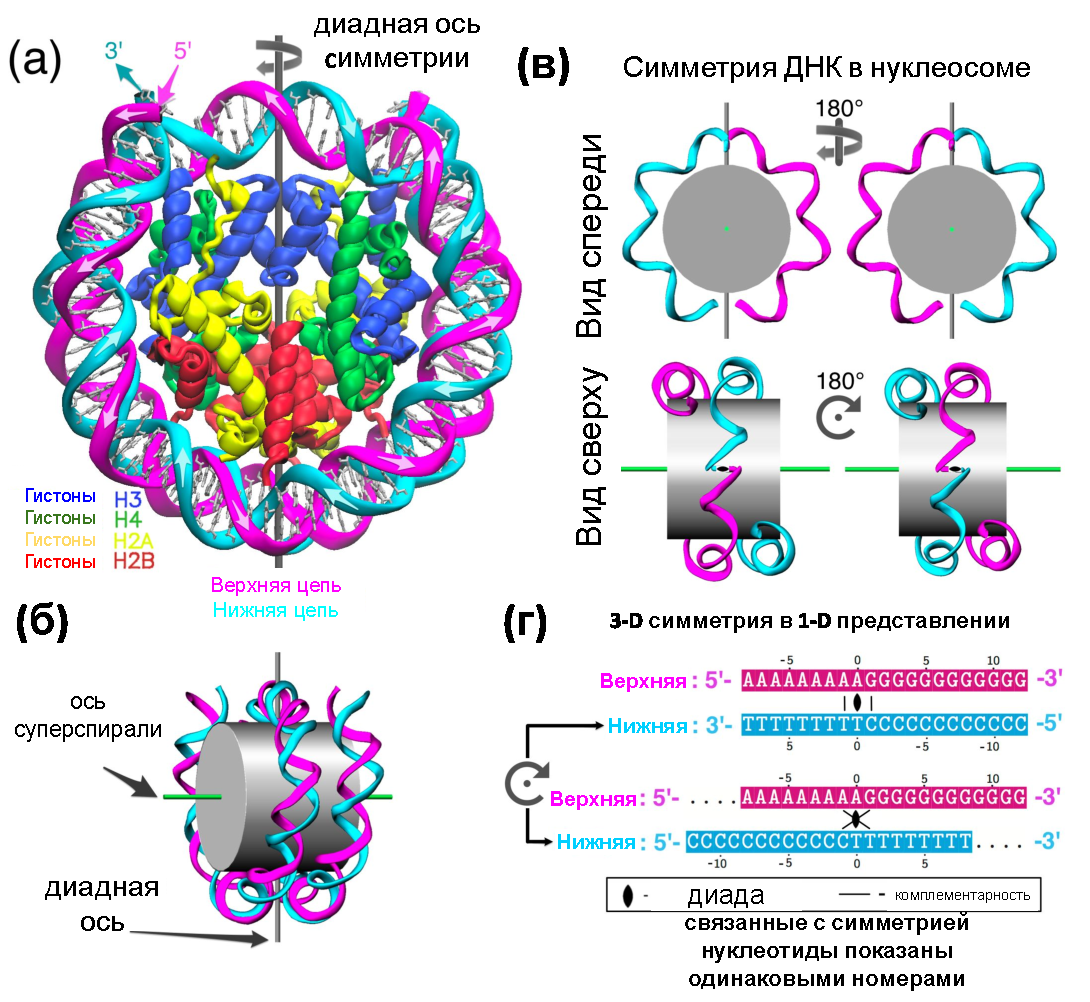
\includegraphics[width=\textwidth]{images/p5/part5_2_nar/p5_2_f1.pdf}
\caption[Структура нуклеосом и псевдосимметрия верхней и нижней цепей ДНК.]{
Структура нуклеосом и псевдосимметрия верхней и нижней цепей ДНК. (а) Представление структуры нуклеосомного кора (PDB 1KX5 (\cite{davey_solvent_2002})). (б) Схематическое изображение нуклеосомы, показывающее расположение оси псевдосимметрии второго порядка и сверхспиральной оси. (в) Иллюстрация псевдосимметричного отношения между верхней и нижней цепями ДНК в нуклеосоме (показаны только части цепей ДНК). (г) Изображение пространственной симметрии ДНК на плоских диаграммах последовательности: обычное представление (вверху) и сонаправленное (внизу). В последнем представлении две нити выровнены путем размещения диадных нуклеотидов верхней и нижней цепей ДНК одного под другим; следовательно, все связанные симметрией пары нуклеотидов верхней и нижней цепей ДНК также выровнены (один под другим). Комплементарность оснований между выбранными нуклеотидами показана на обоих изображениях.}
\label{fig:p5:p5_2_f1}
\end{figure}

\begin{figure}[H]
    \centering
    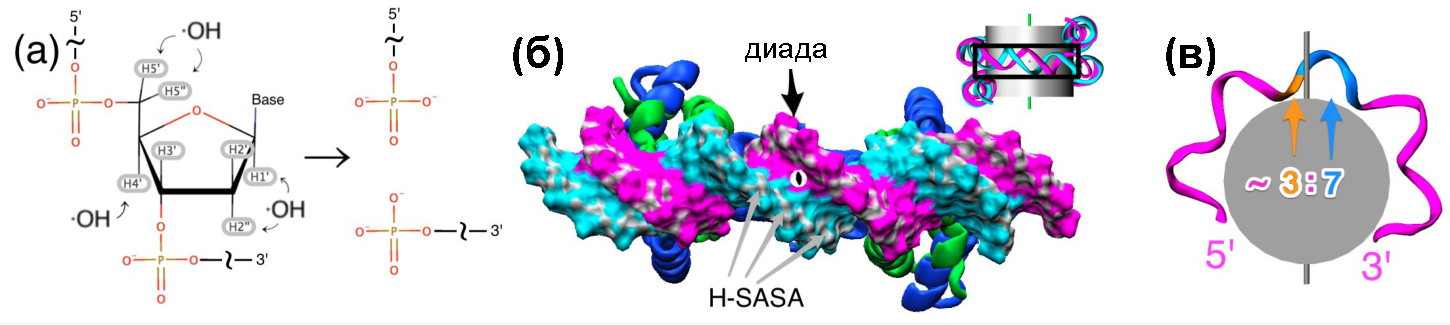
\includegraphics[width=\textwidth]{images/p5/part5_2_nar/p5_2_f2.pdf}
    \caption[Детали гидроксил-радикальных взаимодействий с нуклеосомной ДНК.]{Детали гидроксил-радикальных взаимодействий с нуклеосомной ДНК. (а) Химическая реакция гидроксильных радикалов с основной цепью ДНК: атомы водорода дезоксирибозы (выделены серым) атакуются, что приводит к разрушению остатка дезоксирибозы и расщеплению ДНК. Показаны только основные продукты расщепления. (б) Сегмент нуклеосомы, рассматриваемый сверху (см. Вставку) в представлении площади поверхности, доступной для растворителя (SASA). Участки SASA, принадлежащие атомам водорода дезоксирибозы (H-SASA), окрашены в серый цвет. (в) Асимметрия контактов гистон-ДНК относительно положения оси диады приводит к ее проявлению на профилях расщепления ДНК. Диада делит сегмент цепи ДНК между двумя соседними сайтами связывания на неравные части с соотношением $\sim$ 3:7 при подсчете в направлении 5$^\prime$-3$^\prime$. }
    \label{fig:p5:p5_2_f2}
\end{figure}

\subsection{Материалы и методы}
\subsubsection{Экспериментальные процедуры}

\emph{Приготовление фрагментов ДНК.} ДНК 601-TA была амплифицирована полимеразной цепной реакцией (ПЦР) с асимметричным сайтом рестрикции AvaI, CTCGGG, на обоих концах и клонирована в модифицированный вектор pUC19, который содержит сконструированный асимметричный сайт AvaI. Однако в исследовании ПЦР-амплификация высоко AT-богатой (~ 90\%) центромерной ДНК пекарских дрожжей была проблематичной. Таким образом, фрагмент ДНК CEN3 был химически синтезирован с асимметричным сайтом AvaI и клонирован в вектор pUC57 (Genscript USA Incorporated, Пискатауэй, Нью-Джерси, США). Асимметричный сайт AvaI использовали для лигирования фрагментов ДНК в тандемные массивы. Такие тандемные массивы фрагментов ДНК 601-ТА и центромеры затем клонировали в модифицированном векторе pUC19 с сконструированным асимметричным сайтом AvaI. Для крупномасштабного получения фрагментов ДНК плазмиды, которые содержат тандемные массивы, трансформировали в клетки DH5-$\alpha$ или XL1-Blue для стабильного размножения длинных тандемных массивов фрагментов ДНК. Очищенные плазмиды переваривали рестрикционным ферментом AvaI, и фрагменты очищали электрофорезом в агарозном геле и осаждали этанолом. Нуклеотидный состав четерехнуклеотидного выступа асимметричного сайта AvaI различается между верхней цепью (TS) и нижней цепью (BS), и, таким образом, может использоваться для мечения фрагментов ДНК, специфичных для цепи на 3$^\prime$-конце  с использованием радиоактивно или флуоресцентно меченных нуклеотидов в реакциях с использованием полимеразы Кленова. Поскольку ПЦР проблематична для получения AT-богатого фрагмента центромеры, 5$^\prime$-мечение любого конца потребовало бы химического повторного синтеза ДНК центромеры с дополнительными фланкирующими сайтами рестрикции и создания тандемных массивов для получения крупномасштабной ДНК; по этой причине маркировка 5$^\prime$ не проводилась.

\emph{Подготовка и восстановление нуклеосом}. Экспрессия и очистка коровых гистонов \textit{S. cerevisiae} проводились, как описано ранее \cite{xiao_nonhistone_2011,dyer_reconstitution_2004,mizuguchi_nonhistone_2007}. Октамеры гистонов были восстановлены с использованием известных протоколов \cite{dyer_reconstitution_2004}. Вкратце, эквимолярные количества очищенных рекомбинантных гистонов (H2A, H2B, Cse4 и H4) растворяли в денатурирующем буфере (7M гуанидин-HCl, 20 мМ трис-Cl, pH 7,5, 10 мМ дитиотреитол (ДДТ)) в концентрации 2 мг/мл. Смеси диализовали против четырех замен по 2 литра каждого буфера для рефолдинга (10 мМ Трис-Cl, pH 7,5, 1 мМ ЭДТА, 5 мМ бета-меркаптоэтанол, 0,1 мМ фенилметилсульфонилфторид (ФМСФ)), содержащий 2 М NaCl в течение 2 дней при $4^{\circ}$C. Затем смесь центрифугировали при 15 000 об / мин в микроцентрифуге Tomy MX-300 для удаления любого нерастворимого материала. Растворимые октамеры очищали фракционированием по размеру на колонке для гель-фильтрации Superdex 200. Фрагмент ДНК 601TA 157 п.н. \cite{cloutier_dna_2005} и фрагмент ДНК CEN3 136 п.н. получали, как описано ранее \cite{xiao_nonhistone_2011}. Их полноразмерные последовательности представлены на оси последовательностей на всех соответствующих рисунках. Для воссоздания нуклеосом очищенные октамеры гистонового кора и ДНК смешивали в 50 мкл высокосолевого буфера (2M NaCl, 10 мМ Tris-Cl, pH 7,5, 1 мМ EDTA, 0,02\% NP-40, 5 мМ бета-меркаптоэтанола) с добавлением бычьего сывороточного альбумина 400 мкг / мл. Смесь переносили в диализную установку SlideA-Lyzer MINI (Thermo Scientific). Блок для диализа помещали в контейнер с 600 мл высокосолевого буфера и диализовали в течение 30-60 минут с последующим диализом в солевом градиенте, в течение которого низкосолевой буфер (100 мМ NaCl, 10 мМ трис-Cl, pH 7,5, 1 мМ ЭДТА, 0,02\% NP-40, 2 мМ бета-меркаптоэтанол) закачивали в контейнер со скоростью 3,5 мл / мин в течение 16 часов. Затем диализный блок переносили в буфер с низким содержанием соли и диализовали в течение 60 мин. Диализ проводили при комнатной температуре, а образцы дополнительно обрабатывали при $65^{\circ}$C в течение ночи. 

\emph{Гидроксильный футпринтинг}. Нуклеосомы собирали на основе фрагментов ДНК, меченных по 3$^\prime$-концам с помощью $^{33}$P-dTTP для верхней цепи и $^{33}$P-dATP для нижней цепи, путем заполнения асимметричного сайта AvaI с использованием полимеразы Кленова. HRF нуклеосом выполняли на нуклеосомах с помощью реагента железо (II)-EDTA, как описано ранее \cite{schwanbeck_spatial_2004}. Продукты реакции разделяли на 1,3\% нативном агарозном геле, полосы, содержащие свободные нуклеосомы, визуализировали с помощью окрашивания SYBR Green и вырезали из геля. ДНК выделяли из срезов геля и разделяли на 8\% геле для секвенирования ДНК (National Diagnostics, каталожный номер EC-833). Маркерами подвижности ДНК были реакции секвенирования G + A и C + T тех же $^{33}$P-меченных фрагментов ДНК, которые выполнялись, как описано в Molecular Cloning, CSHL. Гели запускали на 40-сантиметровой стеклянной пластине при 1500-1600 В в течение ~70 минут при температуре геля около $55^{\circ}$C, затем переносили на фильтровальную бумагу DEAE (бумага для ионообменной хроматографии Whatman Grade DE81 от GE Life Sciences) и сушили под вакуумом. Радиоактивные сигналы регистрировались с помощью PhosphorImager (Fuji Photo Film Co., Ltd) и сканера Typhoon (Typhoon 9410, Amersham Biosciences).

\subsubsection{Вычислительный анализ}
\emph{Количественная оценка изображений гелей в экспериментах по футпринтингу гидроксильными радикалами}. Профили интенсивности 1D дорожек для каждой дорожки в геле были извлечены с помощью ImageJ v. 1.51f \cite{schneider_nih_2012}. Линия или ломанная линия была проведена вручную через центры всех полос в дорожке. Ширина линии была установлена примерно на половину ширины дорожки, а профиль сигнала вдоль полосы был извлечен и сохранен в отдельный файл для дальнейшей обработки. Эта стандартная процедура автоматически запускает выпрямление изображения для каждой полосы и усреднение данных по ширине полосы, как это реализовано в ImageJ. Профили интенсивности полос, соответствующие экспериментам с гидроксильными радикалами, были дополнительно проанализированы с помощью нашего недавно разработанного пакета HYDROID (доступного по адресу \url{https://github.com/ncbi/HYDROID}) (публикация в стадии подготовки), чтобы получить значения интенсивности расщепления ДНК. в каждой позиции в последовательности ДНК. Хотя наша методология основана на идеях, предложенных в более ранних работах \cite{shadle_quantitative_1997,takamoto_semi-automated_2004,das_safa_2005}, она имеет несколько новых аспектов. Во-первых, начальные местоположения пиков интенсивности, соответствующих полосам геля, были полуавтоматически назначены и сопоставлены с положениями вдоль последовательности ДНК путем сравнения их с полосами, полученными в результате реакций Максама-Гилберта \cite{jain_footprinting_2008-1}. Диапазон данных на каждом профиле HRF был установлен на область, в которой можно было идентифицировать непрерывный набор отдельных положений полос (либо непосредственно по наличию пика, либо иным образом однозначно выведенный из положения соседних пиков или соответствующих положений полос на других дорожках геля). Затем аналитическая функция была использована для аппроксимации экспериментального профиля HRF. Он представляет собой линейную комбинацию функций Гаусса, каждая из которых предназначена для описания формы определенной полосы на экспериментальном профиле. Алгоритм аппроксимации на основе метода наименьших квадратов Левенберга-Марквардта был использован для решения данной задачи. Параметры ширины функций Гаусса были ограничены, чтобы обеспечить монотонное уменьшение ширины с увеличением молекулярной массы расщепленных фрагментов ДНК, соответствующих полосам геля. Было показано, что такая регуляризация увеличивает точность процедуры аппроксимации и выполняется функцией, реализованной в HYDROID. Ранее функции Лоренца вместо функций Гаусса использовались в качестве эмпирического приближения для уменьшения искажений сигнала из-за авторадиографического метода детекции сигнала в геле (\cite{shadle_quantitative_1997} и приложение к нему). В нашем случае моделирование с помощью функций Лоренца дало несколько худшие результаты, измеренные по среднеквадратическому отклонению между аппроксимированными и экспериментальными кривыми, что оправдывает использование функций Гаусса для нашего анализа. В результате частоты расщепления ДНК для каждой позиции в последовательности ДНК были получены из значений коэффициентов (полученных интегрированием по интенсивностям для каждой полосы) перед функциями Гаусса, описывающими соответствующую полосу. Следует отметить, что профили интенсивности расщепления ДНК обычно различаются по абсолютной величине из-за их зависимости от многих экспериментальных условий (загрузка образца, время воздействия и т. д.). Чтобы обеспечить адекватное сравнение двух экспериментальных профилей, они должны быть в одном масштабе. С этой целью мы выполнили линейную регрессию, описав один профиль HRF как линейную функцию (без свободного члена) другого профиля. Значения последних значений профиля интенсивности затем были масштабированы с помощью полученного коэффициента линейной регрессии и нормализованы от нуля до единицы путем деления на максимальное значение интенсивности двух профилей. Для сравнения экспериментальных и теоретических (H-SASA, определение см. ниже) профилей использовалась простая нормализация каждого профиля по его максимальному значению.

\emph{Молекулярное моделирование и моделирование молекулярной динамики нуклеосом}. Моделирование молекулярной динамики (МД) различных нуклеосом было выполнено в соответствии с нашим протоколом, описанным в работе \cite{shaytan_coupling_2016} если не указано иное. Первоначальные модели были основаны на рентгеновских структурах, полученных из банка данных PDB, или на моделя созданных по гомологии. Первоначально структуры были ориентированы в системе координат нуклеосомы, как определено ранее \cite{shaytan_coupling_2016}, так что ось Z соответствовала суперспиральной оси ДНК (рис. \ref{fig:p5:p5_2_f1}Б). Моделирование проводилось в течение 80 нс, и моментальные снимки сохранялись каждые 1 нс, первые 30 нс МД моделирования отбрасывались как период релаксации. Атомы оснований N1 и N9 в ДНК были привязаны к их исходным положениям с помощью гармонических ограничений с константой жесткости в 6 ккал / моль / A$^2$. Кроме того, мы сравнили МД-траектории с микросекундной траекторией нуклеосомы с полными гистоновыми хвостами и без ограничений на ДНК опубликованой ранее \cite{shaytan_trajectories_2016}. Структуры были визуализированы и проанализированы с использованием VMD \cite{humphrey_vmd_1996}. Первоначальная структура центромерной нуклеосомы \textit{S. cerevisiae} содержащей белок Cse4p с последовательностью ДНК 601TA (601TA-NUC) была построена на основе структуры нуклеосомы \textit{X. laevis} с 601-ой ДНК (PDB ID: 3LZ0) с использованием Modeller \cite{sali_comparative_1993} и 3DNA. Последовательности гистонов были получены из базы данных HistoneDB 2.0 \cite{draizen_histonedb_2016}. Модель центромерной нуклеосомы дрожжей на последовательности ДНК CEN3 (CEN3-NUC) была построена с использованием тех же методов на основе структуры нуклеосомы \textit{X. laevis} с $\alpha$-сателлитной  ДНК (PDB ID: 1KX5). Поскольку нет данных о позиционировании ДНК для этой нуклеосомы, мы определили его, используя наш метод определения диады, примененный к экспериментальным данным HRF для CEN3-NUC (см. ниже). В обеих моделях ДНК моделировали с использованием центрального фрагмента длиной 120 п.н. (60 п.н. от диады в каждом направлении) - фрагмента, который, как известно, однозначно организован центромерными нуклеосомами \cite{tachiwana_crystal_2011}. 

\emph{Теоретическая оценка частотных профилей расщепления ДНК по атомным структурам}. Как предложено в  \cite{balasubramanian_dna_1998}, профили частоты расщепления нуклеосомной ДНК были теоретически оценены как сумма площадей, доступных для растворителя (SASA) для всех атомов водорода дезоксирибозы данного нуклеотида, в дальнейшем называемые профилями H-SASA. Расчеты SASA были выполнены с использованием программы NACCESS \cite{hubbard_naccess_1993} с радиусом зонда 1,4 A, шириной среза 0,005 A и радиусами атомов, установленными в параметрах rmin силового поля CHARMM36 \cite{best_optimization_2012}. Для систем с усеченными гистоновыми хвостами хвосты были усечены в следующих N-концевых (H3G44, H4D24, H2A16T и H2BR33) и C-концевых (H2AK118) положениях (нумерация остатков дана в системе отсчета канонических гистонов \textit{X. laevis}. По умолчанию профили H-SASA были усреднены по 50 снимкам МД (с интервалом каждые 1 нс) полностью гидратированных структур (по причинам, описанным в разделе ``результаты''). Для моделирования МД атомы водорода добавлялись в ходе подготовки системы к моделированию, а в случаях прямого анализа рентгеновских структур положения атомов водорода генерировались с помощью REDUCEv.3.14 из AmberTools13 \cite{word_asparagine_1999}. Графики профилей вместе с последовательностями были созданы с помощью ggplot \cite{wickham_ggplot2_2009} и TexShade \cite{beitz_texshade_2000}. Усечение гистоновых хвостов и релаксация структуры и усреднение, обеспечиваемые моделированием МД, сыграли важную роль в получении профилей H-SASA, которые отражали периодичность ДНК в нуклеосомах (см. Раздел ``Результаты''). Вклад контактов ДНК-белок в профили H-SASA оценивали путем расчета профилей H-SASA для нуклеосомной ДНК с удаленными гистонами. Можно видеть, что модель H-SASA чувствительна к сужению малой бороздки ДНК в определенных местах ДНК-гистоновых взаимодействий, где ДНК изгибается в сторону малой бороздки. Однако контакты гистон-ДНК вносят основной вклад в минимумы H-SASA на этих сайтах.

\emph{Расчет параметров геометрии ДНК}. Параметры, которые представляют пространственную ориентацию, конформацию и периодичность нуклеосомной ДНК в виде одномерных профилей, являются важными инструментами нашего анализа. В качестве основного параметра, отражающего ориентацию пар оснований ДНК в нуклеосомной суперспирали, мы использовали величину относительного кручения нуклеосомной ДНК (relative twist, rTw). Два типа параметров кручения для характеристики суперспиральной ДНК в нуклеосоме были определены ранее: внутреннее кручение (iTw) и rTw (или локальное кручение) \cite{richmond_structure_2003,travers_dna_1993}. Предполагается, что последний измеряется в экспериментах по HRF или ферментативному расщеплению, потому что он подчеркивает геометрически эквивалентные положения вдоль суперспирали ДНК. iTw, с другой стороны, выделяет только собственное вращение пар оснований относительно друг друга вдоль ДНК. Однако известно, что значения rTw и iTw связаны через сверхспиральный шаг нуклеосомной ДНК \cite{travers_dna_1993}. Значения iTw для каждого шага пары оснований были рассчитаны с использованием 3DNA \cite{lu_3dna_2008}; суммирование этого значения по последовательности ДНК дало совокупное значение iTw (ciTw). Чтобы охарактеризовать rTw, мы вводим здесь новую величину - угол ориентации пары оснований (BPOA), предназначенный для отражения локальной ориентации нуклеотидов относительно октамера гистонов. BPOA был рассчитан из атомистических структур нуклеосом следующим образом: (i) суперспиральная ось нуклеосомы (рис. \ref{fig:p5:p5_2_f1}Б) была определена, как описано в работе \cite{shaytan_coupling_2016}; (ii) для каждого нуклеотида был определен вектор пары оснований (BPV) как вектор, указывающий от гликозидного атома азота текущего нуклеотида к соответствующему атому комплементарного нуклеотида (таким образом соединяя атомы N1 и N9); (iii) для каждого нуклеотида его соответствующий центр пары оснований (BPC) определяли как среднюю точку BPV; (iv) BPOA затем определяли как угол между BPV и перпендикуляром, направленным от суперспиральной оси нуклеосомы к BPC (радиальный вектор в цилиндрической системе координат). Значения BPOA служили мерой rTw в диапазоне от 0 до 180$^\circ$. По аналогии с ciTw, кумулятивная rTw (crTw) была реализована путем суммирования вращения BPV вдоль последовательности и добавления 180$^\circ$ каждый раз, когда значение BPOA начинало новый интервал. Относительную (локальную) периодичность нуклеосомной ДНК в каждом конкретном положении рассчитывали на основе разницы значений crTw между сайтами на 5 п.н. выше и ниже выбранного положения. Альтернативный способ расчета rTw с использованием BPOA, определяемого как угол между BPV и плоскостью, перпендикулярной супспиральной оси, дал почти идентичные результаты, что подтвердило наш выбор BPOA в качестве меры rTw. Разница между crTw и ciTw наблюдалась в соответствии с теоретическими ожиданиями. Мы использовали параметр rTw для характеристики пути ДНК в атомистических структурах NCP и для расчета локальной периодичности вдоль последовательности ДНК. Это позволило нам подробно проанализировать вращательное позиционирование ДНК в нуклеосомах и идентифицировать геометрически эквивалентные положения относительно поверхности октамера. Минимумы кривой rTw соответствуют положениям, в которых соответствующие пары оснований ориентированы почти перпендикулярно сверхспиральной оси, а нуклеотид верхней цепи ДНК взаимодействует с октамером главным образом через его атомы основной цепи. Локальная периодичность ДНК для анализируемых структур (рисунки \ref{fig:p5:p5_2_f3}A и \ref{fig:p5:p5_2_f4}) колеблется между 10 и 11 п.н. на оборот, а ДНК чрезмерно скручена вокруг положений $\pm$20 и $\pm$50 (SHL $\pm$2 и $\pm$5), что находится в согласии с результатами статьи \cite{tan_nucleosome_2011}.


\subsection{Результаты}
\subsubsection{Анализ теоретических частотных профилей расщепления ДНК для разных нуклеосом}
Расчет теоретических профилей частоты расщепления HRF основан на предположении, что он определяется профилями HSASA (см. Раздел ``Материалы и методы'') \cite{jain_footprinting_2008-1}. Это, конечно, только приближение к сложным процессам диффузии и взаимодействия, происходящим во время реакции гидроксильного футпринтинга. Однако есть определенные соображения в пользу такого подхода. Это позволяет надежно оценить теоретические профили с разрешением до одиночных нуклеотидов на основе атомных нуклеосомных структур или точных структурных моделей и сделать важные выводы об ожидаемой форме и сходстве экспериментальных профилей. Мы утверждаем, что симметрия нуклеосом может быть использована, чтобы обеспечить способ проверки и повышения точности теоретических профилей, облегчить интерпретацию экспериментальных профилей HRF и позволить идентифицировать диаду нуклеосом из экспериментальных данных HRF. Действительно, нуклеосомы обладают осью псевдосимметрии второго порядка (рис. \ref{fig:p5:p5_2_f1}Б-Г), которая связывает верхнюю и нижнюю цепи нуклеосомной ДНК таким образом, что если нуклеосома повернута на $180^{\circ}$ вокруг оси диады, то верхняя цепь ДНК почти точно совпадет с положением нижней цепи и наоборот. В частности, 5$\prime$-конец верхней цепи будет совмещен с 5$\prime$-концом нижней цепи. Сначала мы исследовали структуру с самым высоким разрешением (PDB ID: 1KX5 \cite{davey_solvent_2002}), где симметрия октамера гистонов дополняется симметрией квазипалиндромной последовательности ДНК: центральная пара оснований на диаде подразделяет нуклеосому и двухцепочечную ДНК на две идентичные половины. В случае известных структур точное положение диады можно непосредственно рассматривать как единственную пару оснований, расположенную на оси псевдосимметрии \cite{luger_crystal_1997}. На рис. \ref{fig:p5:p5_2_f3} показана четкая картина периодичности профилей H-SASA, рассчитанных на основе этой структуры для обеих цепей ДНК. Эта форма и периодичность очень похожи для обеих цепей ДНК, учитывая симметрию системы. Ось диады делит сегмент между двумя минимумами на графике H-SASA на неравные части (примерно в соотношении 3:7) с расположением диады ближе к 5$^\prime$ концу цепи ДНК. Это является следствием геометрии нуклеосомы и проиллюстрировано на рисунках \ref{fig:p5:p5_2_f2}Б и В. На рисунке \ref{fig:p5:p5_2_f3}В профиль H-SASA имеет отчетливые резкие минимумы в каждой позиции, где ДНК ориентирована перпендикулярно поверхности октамера, и довольно похожие на плато области высоких значений подверженности потенциальной атаке гидроксильных радикалов между этими позициями. Расстояние между минимумами на профиле H-SASA соответствует периодичности 10–11 п.н., но положения минимумов H-SASA не всегда точно соответствуют положениям минимумов rTw - они обычно отклоняются на 1 или 2 позиции в любом направлении. Последнее подчеркивает тот факт, что не только кручение ДНК отвечает за точную форму профилей H-SASA, но и различия во взаимодействиях белок-ДНК в различных сайтах связывания ДНК на нуклеосомах влияют на локальные положения минимумов H-SASA. Чтобы получить представление об этих вариациях, мы рассчитали индивидуальный вклад аминокислот в защиту ДНК от гидроксильных радикалов, рассчитанный как изменение общего H-SASA после удаления одного определенного аминокислотного остатка. Хорошим примером локального изменения формы H-SASA является повышенная защита в профилях в положении -43, проявляющаяся в виде локального минимума на рисунке \ref{fig:p5:p5_2_f3}В, который вызван взаимодействиями ДНК с $\alpha$N-спиралью, уникальной для H2A. Несмотря на наличие локальных выбросов, общие профили H-SASA двух цепей ДНК демонстрируют хорошую суперпозицию. Как упоминалось ранее, это результат почти идеальной симметрии данной нуклеосомы как на уровне белка, так и на уровне ДНК. Эксперименты HRF проводятся в растворе на ансамбле нуклеосом, которые в совокупности представляют конформационное пространство, доступное отдельным нуклеосомам в течение длительных периодов времени, поэтому уместно предположить, что две идентичные копии гистонов и хвостов гистонов будут исследовать неразличимые ансамбли конформаций. Следовательно, введенное выше правило симметрии должно также соблюдаться. Гибкие гистоновые хвосты, которые часто встречаются в адсорбированных конформациях в структурах рентгеновских нуклеосом (если они разрешены) могут вносить асимметрию в профиль H-SASA и могут обеспечить значительную дополнительную защиту ДНК от расщепления. Мы обнаружили, что наилучшее совпадение профилей H-SASA, соответствующих двум нитям ДНК были получены, когда гибкие гистоновые хвосты были опущены и ансамблевое усреднение и релаксация остова ДНК была выполнена в ходе МД моделирования (Рисунок \ref{fig:p5:p5_2_f3}В). По этой причине мы реализовали протокол с использованием систем с усеченными гистоновыми хвостами и усреднение по ансамблю МД, который мы использовали на протяжении всего исследования. Далее мы проанализировали влияние вариаций последовательности ДНК на геометрию ДНК и теоретические H-SASA профили. Рисунок \ref{fig:p5:p5_2_f4} суммирует различия в геометрии ДНК и периодичности для трей доступных рентгеновских структуры нуклеосомного кора с разной ДНК последовательностью: $\alpha$-сателлитная ДНК длиной 146 п.н.  (``NCP146'') \cite{luger_crystal_1997}, модифицированная $\alpha$-сателлитная ДНК длиной 147 п.н. (``NCP147'') \cite{davey_solvent_2002}  и 601 высокоаффинная последовательность Видома длиной 145 п.н. (``NCP145'') \cite{lowary_new_1998,vasudevan_crystal_2010}. Во всех этих структурах одна пара нуклеотидов расположена строго на диаде и ДНК проходит один и тот же сверхспиральный путь, несмотря на различия в их длине. Это достигается за счет растяжения/сжатия ДНК на участках, расположенных на расстоянии $\pm$20 или $\pm$50 п.н. от диады. Это иллюстрируется относительной периодичностью параметра rTw, предложенного в этом исследовании (рис. \ref{fig:p5:p5_2_f4}, верхний график). В то время как молекулы ДНК из NCP147 и NCP145 принимают очень похожие конформации с обеих сторон нуклеосомы, ДНК из NCP146 растянута на 1 п.н. с одной стороны. Практически идентичная конформация ДНК по обе стороны диады в NCP147 и NCP145 приводит к очень хорошему наложению между профилями H-SASA для обеих нитей ДНК (коэффициент корреляции Пирсона = 0,97, Рисунок \ref{fig:p5:p5_2_f3}). Что касается NCP146, несмотря на небольшую асимметрию двух половин нуклеосомной ДНК, сходство профиля H-SASA между двумя цепями поддерживается в пределах $\pm$20 п.н. вблизи диады. Однако небольшая асимметрия NCP146 не будет проявляться на профилях HRF для ансамбля нуклеосом в растворе. На самом деле, NCP146, имеющая чисто палиндромную последовательность ДНК, не будет иметь предпочтений относительно того, с какой стороны нуклеосомной ДНК растягиваться или расширяться, потому что две половинки ДНК полностью идентичны.

\begin{figure}[H]
    \centering
    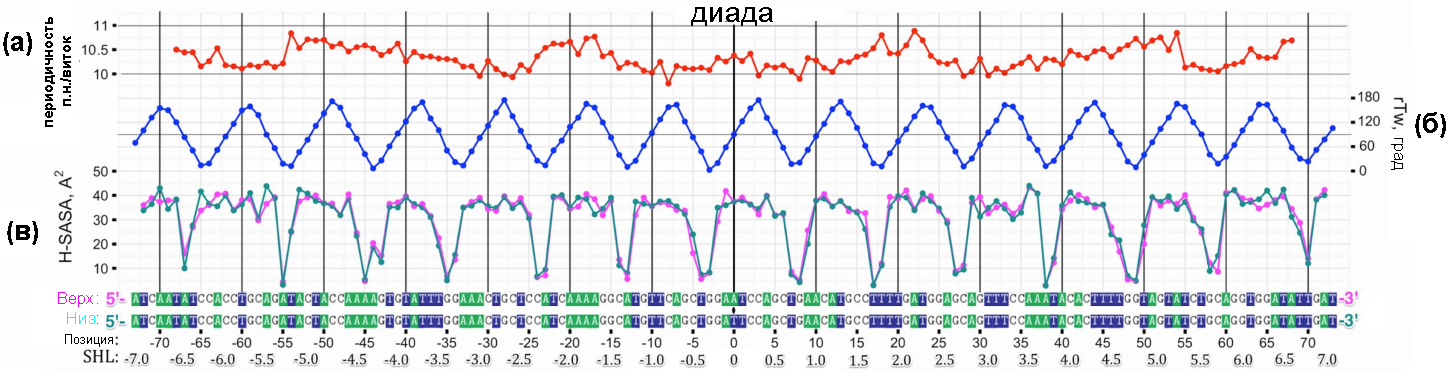
\includegraphics[width=\textwidth]{images/p5/part5_2_nar/p5_2_f3.pdf}
    \caption[Структура ДНК и профили H-SASA в рентгеновской структуре самого высокого разрешения NCP (NCP147)]{Структура ДНК и профили H-SASA в рентгеновской структуре самого высокого разрешения NCP (NCP147). (А) Локальная периодичность вращения ДНК в нуклеосоме, рассчитанная по относительному повороту (rTw). (Б) rTw нуклеосомной ДНК вдоль последовательности, нанесенный в направлении 5'-3' верхней цепи (TS). (В) Профили H-SASA для верхней цепи (пурпурный) и нижней цепи (голубой), оба профиля и последовательности под ними даны в направлении 5'-3'. Профили H-SASA рассчитаны по МД траектории NCP147 без гистоновых хвостов (см. Раздел ``Материалы и методы'').}
    \label{fig:p5:p5_2_f3}
\end{figure}

\begin{figure}[H]
    \centering
    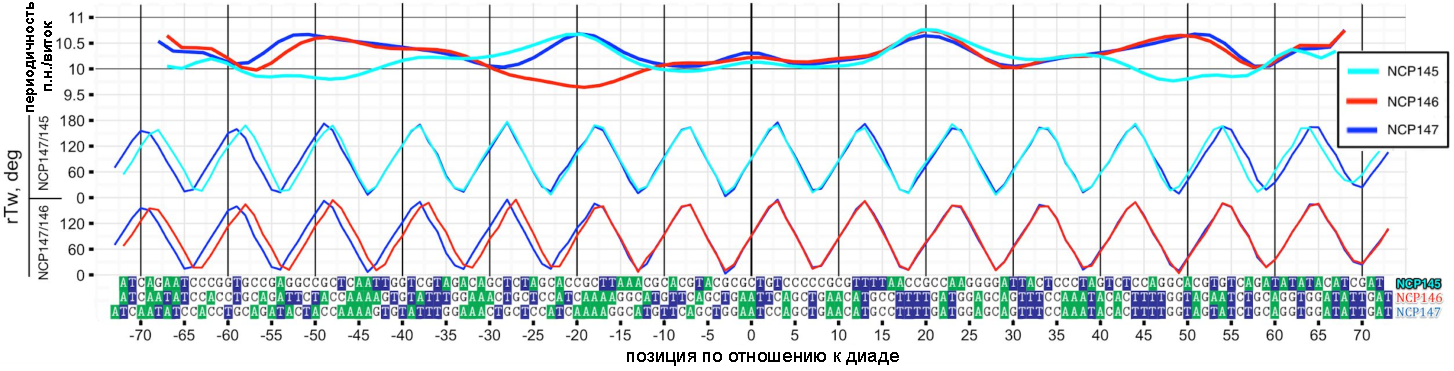
\includegraphics[width=\textwidth]{images/p5/part5_2_nar/p5_2_f4.pdf}
    \caption[Различия в структуре ДНК между разными рентгеновскими структурами нуклеосомы.]{Различия в структуре ДНК между разными рентгеновскими структурами нуклеосомы. Вверху: то же, что на рис. \ref{fig:p5:p5_2_f3}A, но сглаженный B-сплайном (с 30 степенями свободы). Внизу: попарное сравнение профилей rTw.}
    \label{fig:p5:p5_2_f4}
\end{figure}

\subsubsection{Количественная оценка экспериментальных профилей HRF и их сравнение с теоретическими профилями H-SASA}

Мы провели ряд экспериментов по гидроксильному футпринтингу для собранных \textit{in vitro} октамерных нуклеосом  на основе центромерных гистонов \textit{S. cerevisiae} и двух различных последовательностей ДНК: высокоаффинной последовательности 601TA и центромерной ДНК последовательность третьей хромосомы пекарских дрожжей CEN3 (601TA-NUC и CEN3-NUC). Кроме того, мы проанализировали свободную CEN3 ДНК (CEN3-free). Согласно нашей вычислительной процедуре, каждому положению в последовательности ДНК может быть присвоено значение относительной частоты расщепления гидроксильными радикалами путем количественной оценки экспериментально полученного изображения геля ПААГЭ для продуктов реакции HRF (Рисунок \ref{fig:p5:p5_2_f5}). В качестве доказательства концепции на рисунке \ref{fig:p5:p5_2_f5}В изображен экспериментальный профиль HRF 601TA-NUC  по сравнению с теоретическим профилем H-SASA, полученным из модели высокого качества с известной позицией диады созданной на основе рентгеноструктурных исследований (раздел ``Материалы и методы''). Общая периодичность экспериментальных и теоретические профилей хорошо согласуются между собой. Заметное уменьшение амплитуды сигнала к 3$\prime$ концу ДНК, вероятно, связано с пониженной склонностью коротких фрагментов ДНК к осаждению на стадии очистки. Экспериментальные профили для верхней и нижней цепи ДНК при наложении в 5$\prime$–3$\prime$ направлениях (рис. \ref{fig:p5:p5_2_f5}Г) очень похожи по форме, отражая псевдосимметрию нуклеосомы, как показано в предыдущем разделе.

Расположение минимумов в сайтах ДНК-гистоновых взаимодействий на H-SASA и экспериментальных профилях совпадают с точностью до $\pm$1 п.н., в большинстве случаев экспериментальные минимумы смещены к 5$^\prime$-концу цепи по отношению к минимумам H-SASA. Возможное объяснение состоит в том, что во время расщепления гидроксильным радикалом 3$^\prime$- меченой цепи ДНК в дополнение к основному продукту с 5$\prime$-фосфатным концом, как известно, присутствует второстепенный альтернативный продукт - цепь, оканчивающаяся 5$\prime$-альдегидной группой \cite{balasubramanian_dna_1998}. 5$^\prime$-альдегидный продукт, который образуется в результате отрыва 5$\prime$-атома водорода, на 1 нуклеотид длиннее, чем цепь с концевым 5$^\prime$-фосфатным концом, упомянутая выше, и она не имеет отрицательного заряда фосфатной группы и, таким образом, имеет подвижность в геле на 2–3 полосы медленнее по сравнению с соответствующим продуктами реакций Максама – Гилберта \cite{kappen_deoxyribonucleic_1983}. Таким образом, в фактически измеренном профиле частоты расщепления ДНК ожидается, что некоторая часть сигнала будет сдвинута на 2–3 пика в сторону 5$^\prime$-конца. Это может привести к небольшому смещению минимумов на измеренном профиле относительно истинного профиля (аппроксимированного профилем H-SASA). Упомянутый эффект должен быть значительно снижен, если нить ДНК радиоактивно помечена на 5$^\prime$-конце \cite{balasubramanian_dna_1998}, но создание 5-меченых фрагментов центромерной ДНК с высоким содержанием AT является технически сложной задачей (раздел ``Материалы и методы'').

Есть и другие важные различия между теоретически оцененными профилями H-SASA и экспериментальными. Последние демонстрируют гораздо более плавное изменение значений частоты расщепления вдоль последовательности, в то время как профили H-SASA имеют резкие минимумы шириной 1-2 п.н., окруженные областями с высокими значениями частоты расщепления (Рисунок \ref{fig:p5:p5_2_f5}В). Кроме того, хотя в определенных положениях значения H-SASA близки к нулю, что указывает на высокую защиту ДНК от расщепления, экспериментальные данные подтверждают минимальную частоту расщепления по меньшей мере в размере 25\% относительно максимальных значений. В дополнение к этому, экспериментальные профили HRF имеют отчетливые локальные максимумы, которые соответствуют ДНК, обращенной от октамера, в то время как профили H-SASA имеют форму плато в соответствующих областях. Возможные причины этих расхождений указаны в разделе ``Обсуждение'' ниже.

Мы наблюдали, что общий синусоидальный профиль футпринтинга ДНК в нуклеосомах имеет выбросы в определенных положениях пар оснований, их величина варьируется от эксперимента к эксперименту. Эти выбросы лучше всего проиллюстрированы на наборах данных нуклеосом CEN3-NUC и выделены стрелками на рисунке \ref{fig:p5:p5_2_f6}. Интересно, что расположение этих выбросов очень хорошо соответствует положениям выбросов на свободной ДНК. HRF свободной ДНК определяется в основном ее геометрией, которая зависит от последовательности. Необычная природа последовательности CEN3, которая очень богата A-трактами (определяемыми как четыре или более последовательных пары оснований A-T без шага TpA \cite{stefl_dna_2004}), проявляется в виде пиков в местах, где эти A-тракты нарушены гуанинами или цитозинами. Расположение основных пиков, наблюдаемых экспериментально для свободной ДНК CEN3, подтверждается прогнозами веб-сервера ORCHID, который предсказывает профили HRF путем усреднения существующих измерений HRF для всех возможных свободных тринуклеотидов \cite{greenbaum_construction_2007}. Тем не менее, не следует ожидать идеального соответствия между этими двумя методами, поскольку A-тракты характеризуются нелокальными разветвленными водородными связями, которые могут приводить к неаддитивным дальнодействующим, а не локальным эффектам, проявляемым в тринуклеотидах \cite{haran_unique_2009}. Появление аналогичных выбросов на HRF профилях нуклеосомальной ДНК, вероятно, связано с взаимодействием между внутренней геометрией и динамикой свободной ДНК и геометрией, наложенной на ДНК путем связывания с гистонами. Наше моделирование теоретических профилей расщепления с использованием МД-моделирования предполагает, что значения H-SASA довольно чувствительны к небольшим колебаниям двугранных углов основной цепи ДНК, которые могут быть вызваны только небольшими смещениями положений пары оснований. Это дает один потенциальный ключ к пониманию того, как небольшие изменения в структуре и динамике нуклеосом из-за вариации последовательности ДНК могут проявляться в профилях HRF.


\subsubsection{Новый метод определения положения нуклеосомной ДНК на основе данных гидроксильного футпринтинга}
Анализ как экспериментальных профилей, так и профилей H-SASA, описанных в предыдущих разделах, выявил несколько ключевых взаимосвязей между формой профилей HRF и положением ДНК на нуклеосоме. Описанный ниже метод идентификации диады основан на этих наблюдениях. Ось псевдосимметрии воторого порядка нуклеосомы (рисунок \ref{fig:p5:p5_2_f1}) связывает верхнюю и нижнюю цепи нуклеосомной ДНК так, что если нуклеосома повернута на 180$\circ$ вокруг диадной оси, то верхняя цепь ДНК накладывается на симметричное положение нижней цепи и наоборот (Рисунок \ref{fig:p5:p5_2_f1}В). Это наблюдение подразумевает, что профили HRF для верхней и нижней цепей ДНК должны совпадать (или быть очень похожими в зависимости от степень псевдосимметрии, как обсуждалось ранее), если оба профиля сравнивать в том же направлении (в нашем случае от 5$^\prime$ к 3$^\prime$). На основе H-SASA и экспериментальных профилей HRF, а также анализе геометрии структуры нуклеосомы, можно увидеть, что положение диады расположено асимметрично между двумя локальными минимумами на соответствующем профили любой из нитей ДНК. Диада делит отрезок между минимумами примерно в соотношении 3:7 (далее именуемое ``правилом соотношения 3:7'') (Рисунок \ref{fig:p5:p5_2_f1}В).
Важным аспектом является выбор правильных систем отсчета для сравнения профилей верхней и нижней цепей. Это особенно актуально, поскольку в профилях HRF обычно отсутствуют данные около концов нуклеосомной ДНК из-за ограниченного разрешения ПААГЭ, что делает невозможным идентифицировать нуклеосомную границу на каждом профиле и использовать ее в качестве маркера для их выравнивания. Однако, если известно положение диады в ДНК, также известны положения соответствующих нуклеотидов диады на каждом профиле. В этом случае, из-за геометрических причин и соображений комплементарности оснований цепи, правильный выбор систем отсчета может быть достигнут путем размещения положений нуклеотидов диады каждого профиля в 0, как показано на рисунке \ref{fig:p5:p5_2_f1}Г. Это проиллюстрировано на примере системы 601TA-NUC (рис. \ref{fig:p5:p5_2_f5}Г), где известное положение диады из структуры (см. Раздел ``Материалы и методы'') используется для построения экспериментальных профилей HRF для верхней и нижней цепей ДНК одной и той же системы в их соответствующих системах отсчета. Два профиля выглядят идеально выровненными (коэффициент корреляции Пирсона = 0,94), что подтверждает правильный выбор положения диады.
Если теперь представить себе ситуацию, когда положение диады неизвестно, но есть эксперименты по гидроксильному футпринтингу для обеих цепей ДНК, описанный выше подход можно легко обобщить для определения положения диады и, следовательно, общего позиционирования ДНК (также называемого позиционированием нуклеосом). Поскольку каждое значение интенсивности профиля HRF соответствует определенному основанию на цепи ДНК, выравнивание профиля определяет выравнивание последовательностей двух цепей, нанесенных на график в направлении от 5$^\prime$ к 3$^\prime$. Соответствующее положение диады на выравнивании последовательностей между верхней и нижней цепями ДНК затем может быть идентифицировано как единственное положение, где выровненные основания образуют пару оснований в структуре двухцепочечной нуклеосомной ДНК.
На практике производится выборка различных совмещений профилей HRF для верхней и нижней цепей ДНК, и качество их соответствия оценивается путем вычисления коэффициента корреляции между двумя выровненными профилями HRF (только перекрывающиеся части профилей используются для расчета коэффициента). Такой подход вдохновлен теорией обработки сигналов, в которой сходство между двумя процессами оценивается путем вычисления функции взаимной корреляции. Положение диады должно соответствовать максимуму (хотя бы локальному максимуму) коэффициента корреляции. Корреляция между двумя профилями HRF как функция предполагаемого положения диады для данных 601TA-NUC показана на рисунке \ref{fig:p5:p5_2_f7}A. На этом рисунке есть несколько максимумов коэффициента корреляции, разнесенных периодически на ~5 п.н., и в некоторых случаях может быть неоднозначность относительно того, какой максимум соответствует истинному положению диады. Применение ``правила 3:7'' полезно, поскольку половину этих максимумов корреляции можно отбросить как стереохимически ``запрещенные'' диадные позиции. Таким образом можно идентифицировать ``настоящую'' позицию диады (рис.  \ref{fig:p5:p5_2_f7}). Упомянутая периодичность и потенциальная неоднозначность являются следствием (i) квазипериодической природы конформации ДНК в нуклеосоме и (ii) ограниченного диапазона положений в последовательности ДНК, для которых измеряли профиль расщепления ДНК. Однако на практике приблизительное положение диады (например, найденное путем определения местоположения границ нуклеосом посредством расщепления МНКазой) может использоваться для разрешения неоднозначности. В качестве альтернативы можно использовать более длинные профили HRF, которые пересекают границы нуклеосом.
Точность нашего метода явно зависит от качества и отношения сигнал / шум данных. Например, для нуклеосом 601TA-NUC из данных, полученных в этом исследовании, положение диады может быть воспроизведено с точностью до 0,5 п.н. (рис. \ref{fig:p5:p5_2_f7}A). Более высокая точность разрешения по сравнению с одной парой оснований связана с тем фактом, что диада потенциально может быть расположена не только в определенном положении пары оснований, но также между двумя соседними парами оснований, хотя последняя возможность не была замечена в рентгеновских структурах до сих пор. Однако стоит отметить, что положение диады в нуклеосомах в растворе является внутренне статистической характеристикой, и для палиндромных последовательностей ожидается, что среднее положение будет находиться между двумя парами оснований (как обсуждалось ранее для NCP146).
Важно отметить, что наш подход к идентификации диады устойчив по отношению к систематическим экспериментальным ошибкам, например, возникающим из-за минорных продуктов расщепления ДНК, как описано в предыдущем разделе. Эти смещения обычно одинаковы для верхней и нижней цепей, и сходство конформации ДНК в нуклеосоме из-за псевдосимметрии все же должно приводить к подобию экспериментально измеренных профилей расщепления.

\begin{figure}[H]
    \centering
    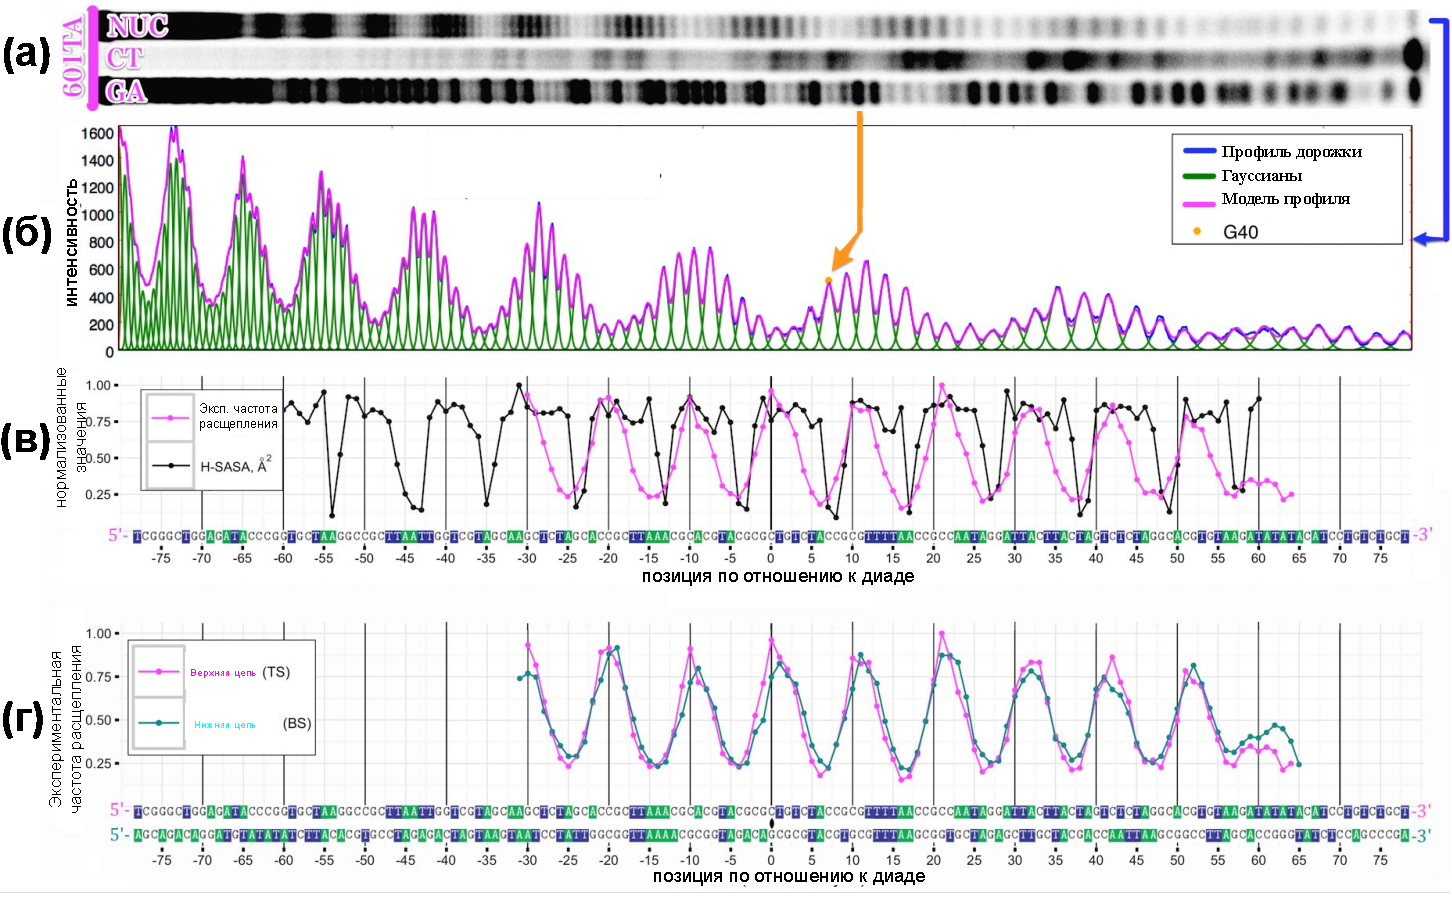
\includegraphics[width=\textwidth]{images/p5/part5_2_nar/p5_2_f5.pdf}
    \caption[Количественная оценка экспериментов по гидроксильному футпринтингу и сравнение с теоретическими профилями, полученными на основе атомной структуры (для нуклеосомы 601TA-NUC)]{Количественная оценка экспериментов по гидроксильному футпринтингу и сравнение с теоретическими профилями, полученными на основе атомной структуры (для нуклеосомы 601TA-NUC). (A) Исходное изображение геля ПААГЭ для сегментов ДНК, полученных с помощью гидроксильного футпринтинга нуклеосом, восстановленных на последовательности 601TA (NUC), и соответствующих продуктов реакции Максама-Гилберта (CT, GA). Данные показаны только для верхней цепи. (Б) соответствующий необработанный профиль интенсивности дорожек HRF, извлеченный из изображения геля, и его деконволюция в индивидуальные интенсивности полос путем подбора функций Гаусса; приводятся среднеквадратическое отклонение (RMSD) и относительное RMSD между исходным профилем и подобранной моделью; также указано RMSD для площади пика, площади пиков рассчитываются как площади под кривой между соседними минимумами. (В) суперпозиция количественных экспериментальных частот расщепления ДНК и профилей H-SASA, рассчитанных на основе атомистической структуры; оба профиля нормализованы до своих максимальных значений. (Г) Суперпозиция экспериментальных частот расщепления ДНК для верхней и нижней цепей ДНК в нуклеосоме 601TA-NUC}
    \label{fig:p5:p5_2_f5}
\end{figure}

\begin{figure}[H]
    \centering
    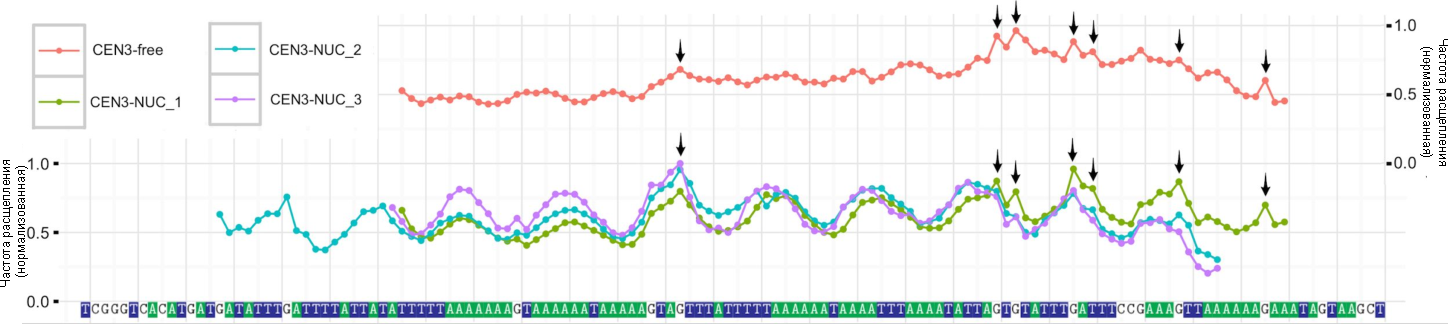
\includegraphics[width=\textwidth]{images/p5/part5_2_nar/p5_2_f6.pdf}
    \caption[Профили частоты расщепления ДНК для нуклеосом CEN3-NUC и ДНК свободной CEN3 ДНК]{Профили частоты расщепления ДНК для нуклеосом CEN3-NUC и ДНК свободной CEN3 ДНК. Данные нескольких экспериментов для верхней цепи объединены, стрелки указывают на незначительные всплески, видимые как на свободных, так и на нуклеосомных профилях ДНК, приписываемые зависимым от последовательности вкладам.}
    \label{fig:p5:p5_2_f6}
\end{figure}



\subsubsection{Моделирование нуклеосомы дрожжей CEN3 помощью интегративного подхода}
Мы использовали метод, описанный в предыдущем разделе, чтобы определить положение диады в восстановленной \textit{in vitro} центромерной нуклеосоме \textit{S. cerevisiae} из хромосомы III (CEN3-NUC) и построить ее структурную модель. С этой целью были проанализированы профили HRF для обеих нитей ДНК, полученные в результате трех независимых экспериментов (рисунок \ref{fig:p5:p5_2_f6}), в соответствии с предложенным нами методом. Мы проиллюстрируем применение нашего подхода к этому набору данных ниже. Были взяты образцы и протестированы различные предполагаемые положения диады нуклеосомы, как описано ранее. Специфическая интерес представляла область вблизи положения 64, которое, как предполагалось в более ранних экспериментах MNase-seq, была центром области устойчивости к расщеплению МНКазой \cite{cole_centromeric_2011}. Корреляционный анализ (рис. \ref{fig:p5:p5_2_f8}A и Б) выявил несколько возможных позиций диад с высокими уровнями корреляции между выровненными профилями (позиции 61,5, 67 и 72). Позиция 67 была отклонена как нарушающая соотношение ``правило 3:7'', что становится очевидным после просмотра выравнивания профилей HRF. Были еще две возможные позиции 61,5 и 72 с одинаковым соотношением коэффициента R = 0,78. Однако позиция 61,5 обеспечила лучшее соответствие между профилями верхней и нижней цепи ДНК в регионе вокруг диады (и, таким образом, ее можно считать лучшим кандидатом для расположения диады). Положение 61.5 расположено намного ближе к нашей исходной области интереса, основанной на оценке положения диады \textit{in vivo} (положение 64).
Все доступные рентгеновские структуры нуклеосом указывают на положение диады на конкретном нуклеотиде, а не между ними. В то же время, как обсуждалось ранее, среднее расположение диады в полуцелом положении возможно для ансамбля нуклеосом в растворе, особенно в случае палиндромных последовательностей. Анализ коэффициента корреляции указал на позицию 61 как более предпочтительную (рис. \ref{fig:p5:p5_2_f8}A), и ее в дальнейшем использовали для построения точной модели нуклеосомы CEN3-NUC (рис. \ref{fig:p5:p5_2_f8}В).
Знание точного местоположения диады позволяет впервые увидеть пространственные отношения между ключевыми элементами ДНК и белковыми элементами, которые определяют функцию центромерных нуклеосом у дрожжей. Как A-участки ДНК, так и ключевые остатки гистона Cse4p, как было показано ранее, являются критическими для функции центромеры у дрожжей, однако их коллективное взаимодействие остается не вполне понятным \cite{baker_genetic_2005,malik_major_2009}.

\begin{figure}[H]
    \centering
    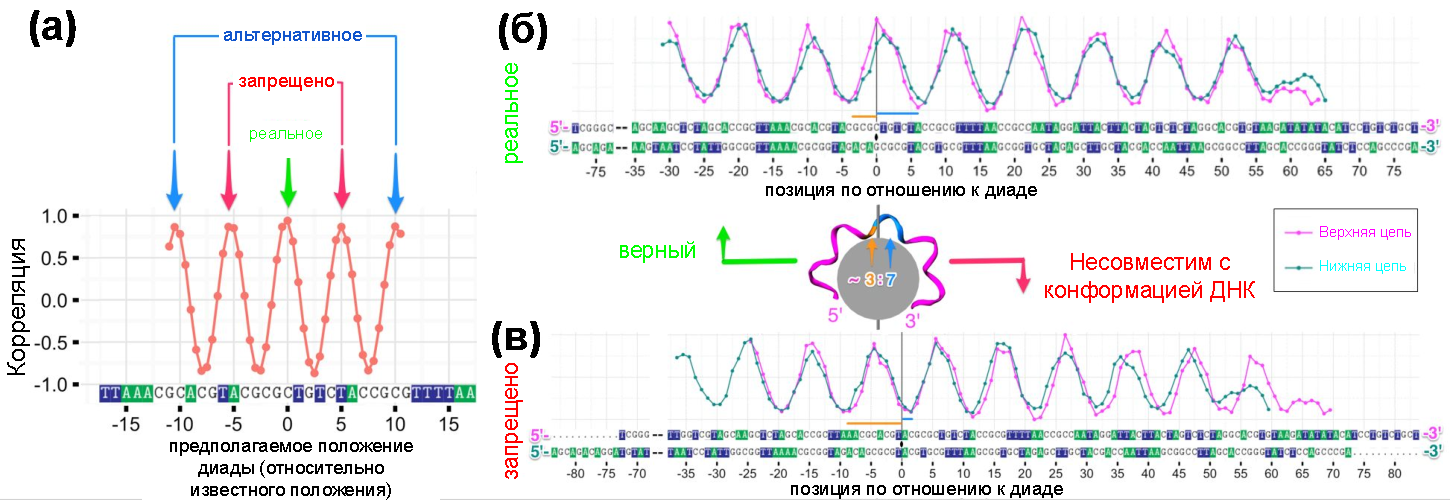
\includegraphics[width=\textwidth]{images/p5/part5_2_nar/p5_2_f7.pdf}
    \caption[Объяснение алгоритма идентификации диады применительно к нуклеосоме 601TA-NUC с известным положением диады]{Объяснение алгоритма идентификации диады применительно к нуклеосоме 601TA-NUC с известным положением диады. (A) Коэффициент корреляции Пирсона между экспериментальными профилями HRF верхней (TS) и нижней (BS) цепей ДНК как функция предполагаемого положения диады, используемого для выравнивания этих профилей. Реальное положение диады соответствует одному из локальных максимумов. Только половина локальных максимумов совместима со стереохимически допустимым решением (``правило 3: 7''). (Б) Наложение профилей TS и BS, выровненных с использованием реальной (известной) позиции диады. (В) Наложение профилей TS и BS, выровненных с использованием стереохимически запрещенного предполагаемого положения диады.}
    \label{fig:p5:p5_2_f7}
\end{figure}


\begin{figure}[H]
    \centering
    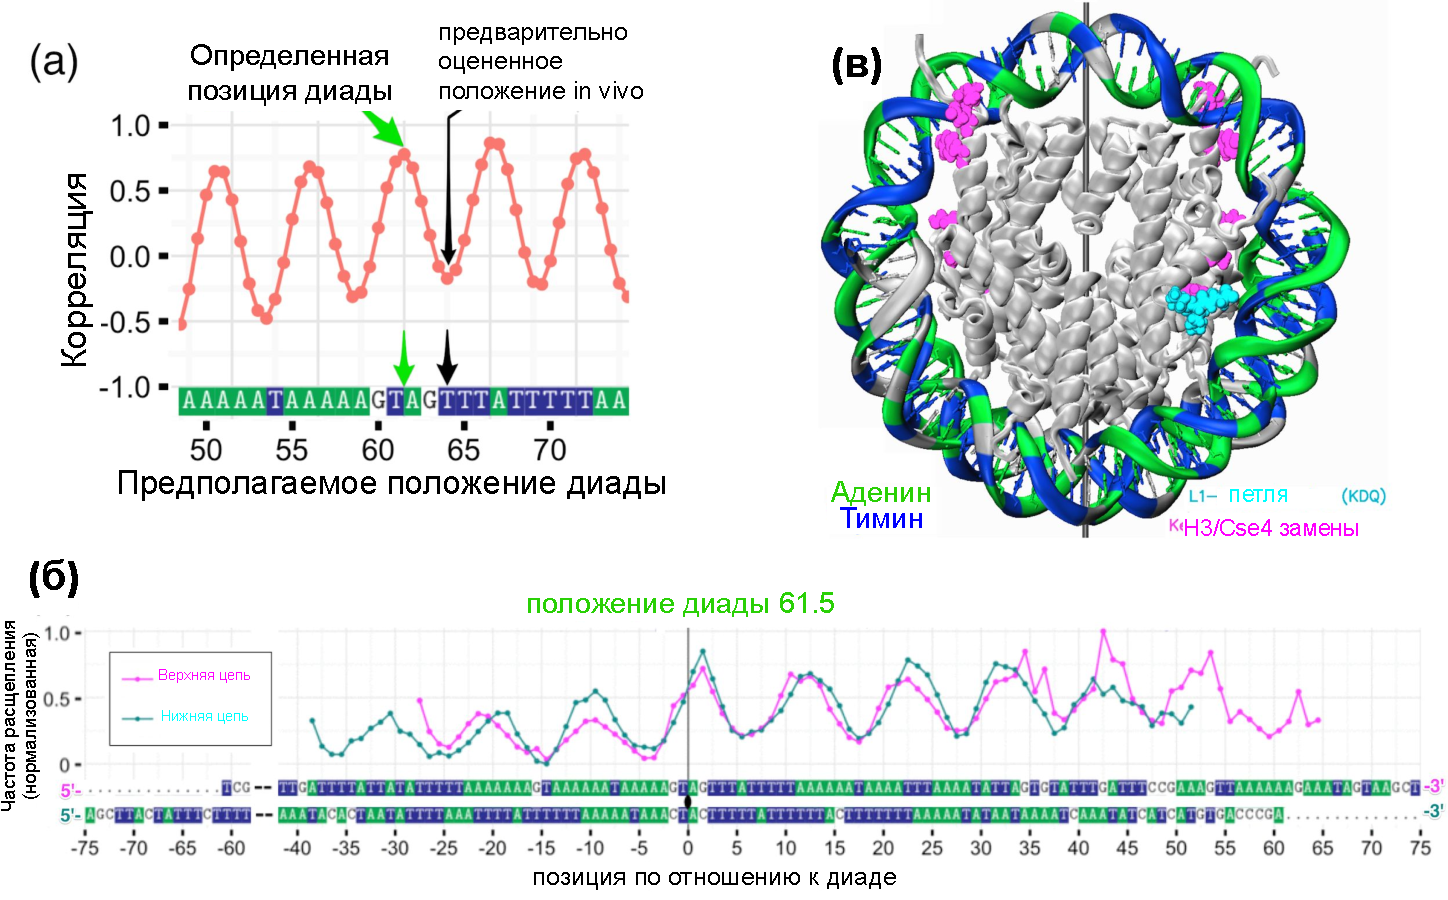
\includegraphics[width=\textwidth]{images/p5/part5_2_nar/p5_2_f8.pdf}
    \caption[Применение алгоритма идентификации диады  к нуклеосоме CEN3-NUC с неизвестным положением диады.]{Применение алгоритма идентификации диады  к нуклеосоме CEN3-NUC с неизвестным положением диады. (A) коэффициент корреляции Пирсона между экспериментальными профилями HRF верхней (TS) и нижней (BS) цепей ДНК как функция предполагаемого положения диады; показано положение диады, согласующееся с данными HRF (зеленая стрелка) и ранее оцененное \textit{in vivo} положение по устойчивости к расщеплению микрококовой нуклеазой (черная стрелка) \cite{cole_centromeric_2011}. (Б) Наложение профилей TS и BS, выровненных с использованием идентифицированной позиции диады. (В) Модель нуклеосомы CEN3-NUC, построенная с использованием положения ДНК, идентифицированного в экспериментах с HRF (диада установлена в положение 61). Нити ДНК окрашены в соответствии с их последовательностью, выделяя AT-участки: A –– зеленый, T –– синий, G или C –– серый.}
    \label{fig:p5:p5_2_f8}
\end{figure}



\subsection{Обсуждение}
В этой работе мы провели эксперименты по гидроксильному футпринтингу на двух нуклеосомных системах и разработали вычислительную основу для анализа данных HRF, полученных в результате экспериментов с нуклеосомами в растворе; интерпретации данных HRF путем сравнения с теоретическими профилями H-SASA; определения точного положение ДНК по данным HRF. Используя расширенный анализ структур нуклеосом, в сочетании с количественной оценкой экспериментальных данных HRF, мы смогли предложить интерпретацию экспериментов HRF на концептуально новом уровне. Это, в свою очередь, привело к развитию простого метода определения положения диады нуклеосом с разрешением в одну пару оснований. Мы использовали этот метод для определения положения диады в реконструированной \textit{in vitro} центромерной нуклеосоме \textit{S. cerevisiae} и для построения ее структурной модели. 
Алгоритм  идентификации диады, предложенный в этом исследовании, основан на соотношении симметрии между двумя цепями нуклеосомной ДНК. Мы показали, что это требование симметрии прямо выражается в сходстве профилей HRF верхней и нижней цепей ДНК. Использование этого критерия и экспериментальных данных для двух цепей ДНК повышает точность и надежность метода идентификации диады по сравнению с ситуацией, когда профиль HRF для каждой цепи анализируется отдельно. Последний подход до сих пор использовался в нескольких предыдущих исследованиях, которые в основном прибегали к сообщению приблизительного местоположения диады на ДНК \cite{hayes_structure_1990,widlund_nucleosome_1999,morozov_using_2009,ober_12-dgpg_2008,cannistraro_rapid_2015}. Идентификация положения диады с разрешением в одну пару оснований ранее достигалась сайт-направленным расщеплением гидроксильными радикалами или сайт-специфическим фотохимическим сшиванием \cite{flaus_mapping_1996,kassabov_high-resolution_2002}. Однако эти методы требуют химического включения определенных зондов в октамер гистонов в симметричных положениях, и диада затем определяется как средняя точка между реакционными сайтами. Метод, описанный в данной работе, обеспечивает разрешение в одну пару оснований с использованием обычных экспериментальных данных HRF без необходимости дорогостоящих модификаций гистонов. 
В качестве доказательства концепции мы оценили расположение ДНК в \textit{in vitro} нуклеосоме CEN3-NUC, которое оказалось на расстоянии ~ 3 п.н. от ранее оцененного положения \textit{in vivo} центра области, устойчивой к расщеплению микрококовой нуклеазе \cite{cole_centromeric_2011}. Точно определенное положение диады позволило нам построить модель этой нуклеосомы и выявить пространственную взаимосвязь между ориентацией последовательности ДНК и ключевыми белковыми мотивами белка Cse4p (Рисунок \ref{fig:p5:p5_2_f8}). Наша модель может служить основой для будущих исследований, направленных на понимание кооперативного взаимодействия и взаимодействия между белком Cse4p и A-траками последовательностей CEN центромер хромосом пекарских дрожжей.
В настоящее время известно, что последовательности CEN не консервативны между разными хромосомами у дрожжей, но наличие в их составе А-трактов имеет решающее значение для выживания \cite{baker_genetic_2005}. Однако молекулярный механизм(ы) вовлечения А-трактов в функцию центромеры дрожжей остается неясным. Одним из аспектов может быть особая геометрия ДНК, присущая А-трактам, которые известны своей конформационной жесткостью и узкими малыми бороздками как в свободной ДНК \cite{haran_unique_2009}, так и в нуклеосоме \cite{bao_nucleosome_2006}. В отличие от обычного гистона H3, вариант Cse4p не имеет остатка аргинина (замещенного серином R63S153), который в случае H3 вставлен в малую бороздку ДНК около положения $\pm$ 15. Известно, что это положение примыкает к уникальному гистоновому мотиву, который формирует чрезвычайно узкую малую бороздку через гидрофобный ``сахарный зажим'' \cite{wu_structural_2010}. С другой стороны, известно, что мотивы TnAn (в отличие от AnTn и в отличие от A-трактов) обнаруживают расширенные малые бороздки на динуклеотидах TpA \cite{stefl_dna_2004}. Последовательности CEN с высоким содержанием AT обычно имеют несколько A-трактов, которые разделены динуклеотидами TpA, и, таким образом, последовательности CEN также содержат несколько TnAn-подобных мотивов. Эти мотивы могут способствовать функционально важному расширению малой бороздки на соответствующих участках.
Интересно, что согласно нашей структурной модели центромерной нуклеосомы, последовательность CEN3 является квазипалиндромной рядом с определенным положением диады 61,5. Последовательность AAAGTAGTTT, обнаруженная на диаде, может быть преобразована в идеальный палиндром с заменой только 1 нуклеотида. Кроме того, 4 нуклеотида в диаде (GTAG) фланкированы сегментами ДНК, состоящими исключительно из A или T, богатых A-участками. Эти структурные данные могут дополнительно обеспечить понимание структуры центромерных нуклеосом и функционального связывания с ключевыми кинетохорными белками, такими как дрожжевой Mif2 (человеческий CENP-C), который предпочтительно связывается с AT-богатыми ДНК центромерных нуклеосом дрожжей (Xiao et al., Неопубликованные данные).

Помимо определения положения диады, эксперименты HRF могут быть использованы для дальнейшего углубления нашего понимания конформации ДНК в нуклеосомах. Возможность сделать это, однако, зависит от нашей способности сопоставить форму профилей HRF со структурными деталями нуклеосомы. Понимание расхождений между теоретически полученными профилями H-SASA и экспериментальными профилями HRF для известных структур является важным шагом в этом направлении. Наш сравнительный анализ профилей H-SASA и экспериментальных профилей показал, что, хотя их общая периодичность схожа, экспериментальные профили намного более гладкие и могут иметь разную величину и / или точное расположение максимумов и минимумов. Разница между теоретическими и экспериментальными профилями также была замечена в предыдущем исследовании комплекса ДНК-ТВР: значения H-SASA для некоторых нуклеотидов были близки к нулю, в то время как определенное количество расщеплений все же было обнаружено экспериментально \cite{pastor_detailed_2000}. Значительная вероятность расщепления ДНК на сайтах связывания ДНК может быть результатом нелинейной зависимости частоты расщепления от доступности растворителю. Фактически, предыдущие исследования показали обнаруживаемые вероятности расщепления за счет отрыва атомов водорода с исчезающе малой SASA \cite{balasubramanian_dna_1998}. Тем не менее, существенный вклад, вероятно, исходит от нуклеосомной динамики и конформационной неоднородности \cite{rychkov_partially_2017,winogradoff_shearing_2015}. Нуклеосомная ДНК в растворе принимает ряд состояний с твист-дефектом ДНК \cite{edayathumangalam_nucleosomes_2005}. В течение HRF экспериментов ансамбль нуклеосом в растворе с различными конформациями будет доступен для гидроксилрадикальной атаки. Дополнительные конформационные вариации также могут быть результатом различий в позиционировании ДНК \cite{widom_role_2001}.

Одним из важных аспектов является появление идентифицируемых локальных максимумов на экспериментальном профиле на расстоянии 10–11 п.н. - по одному на виток нуклеосомной ДНК, тогда как в профилях H-SASA 7–8 нуклеотидов ДНК витка почти одинаково доступны. Возможное объяснение может исходить из несовершенства модели H-SASA, служащей приближением сложной физики и химии разрыва ДНК. В частности, как подчеркивают Бегусова и др. контролируемая диффузией природа реакции атаки гидроксильных радикалов и быстрый распад радикалов из-за взаимодействия с другими атомами должны сделать вероятность разрыва зависимой не только от локальной доступности атомов водорода, но и от общей формы молекулы, которая будет управляют потоком радикалов, которые могут достичь заданного участка ДНК из раствора \cite{begusova_radack_2001,begusova_radiolysis_2000}. Более того, необходимо учитывать распределение электронной плотности целевой молекулы, чтобы правильно описать реакцию атаки гидроксильных радикалов. Различные многоступенчатые реакционные пути могут также вносить вклад в химическую сложность, например, сообщалось о механизмах расщепления ДНК посредством вторичных гистоновых радикалов \cite{zhou_dna_2014}.

С момента пионерских исследований лабораторий Вольфа и Туллиуса в начале 1990-х годов по периодичности нуклеосомной ДНК в растворе на основе экспериментов HRF \cite{hayes_structure_1990,hayes_histone_1991,hayes_histone_1991-1,bashkin_structure_1993} стали доступны рентгеновские структуры нуклеосом с высоким разрешением \cite{luger_crystal_1997}. Периодичность ДНК в нуклеосомах является важным параметром из-за ее влияния на сверхспирализацию ДНК \cite{klug_helical_1981}. Наше исследование, путем одновременного анализа профилей rTw, H-SASA и экспериментальных профилей HRF, позволяет изучить теоретические основы использования экспериментов HRF для определения периодичности ДНК. Результаты нашего анализа в настоящее время требуют осторожности при использовании положений максимумов или минимумов на экспериментальных профилях частоты расщепления ДНК для измерения периодичности нуклеосомной ДНК с высокой точностью (лучше, чем 1 п.н. / оборот). Как мы показали, минимумы профилей на профилях rTw и H-SASA не всегда совпадают, а положения минимумов могут отличаться на 1-2 п.н. из-за вариаций в локальных взаимодействиях гистон-ДНК. С другой стороны, максимумы на экспериментальных профилях частоты расщепления ДНК могут зависеть от локальной динамики ДНК, природы допустимых дефектов кручения, других динамических эффектов, а также некоторых нерегулярностей расщепления, специфичных для последовательности (локальные пики, как показано на рисунке \ref{fig:p5:p5_2_f8}). Кроме того, второстепенные, медленно мигрирующие продукты расщепления ДНК могут исказить форму профилей. Дальнейшие исследования могут выявить вклад этих эффектов в мельчайшие детали формы профилей HRF.

В совокупности наше исследование обеспечивает новый надежный подход к анализу и интерпретации данных экспериментов по расщеплению ДНК нуклеосом гидроксильными радикалами, определению положения ДНК с точностью до одной пары оснований и построению высокоточных молекулярных моделей неизвестных нуклеосом. Такие модели позволяют обнаружить уникальное пространственное расположение между гистонами и особенностями последовательностей ДНК и могут формировать рациональную основу для структурного понимания взаимодействий между нуклеосомами и другими белками хроматина. Учитывая аналогию между HRF и окислительным повреждением ДНК в клетках, результаты этого исследования могут быть в дальнейшем использованы для обоснования влияния нуклеосом на повреждение ДНК с высоким разрешением.



\subsection{Благодарности}
Мы благодарим Т. Туллиуса за ценные предложения, которые помогли сформулировать идею этого исследования, и Л. Заславского за обсуждения оптимальных алгоритмов подбора данных.
Исследования были поддержаны программой очных исследований Национальной медицинской библиотеки и Национального института рака, Национальных институтов здоровья, США; Российским научным фондом [14–24-00031] (договор № 14-24-00031-р, разработка алгоритмов визуализации нуклеосом); Исследовательским кампусом Джанелия Медицинского института Говарда Хьюза;  Университетом Джона Хопкинса; программой сотрудничества США-России в области биомедицинских наук.



